%%%%%%%%%%%%%%%%%%%%%%% file template.tex %%%%%%%%%%%%%%%%%%%%%%%%%
%
% This is a template file for The European Physical Journal
%
% Copy it to a new file with a new name and use it as the basis
% for your article
%
%%%%%%%%%%%%%%%%%%%%%%%% Springer-Verlag %%%%%%%%%%%%%%%%%%%%%%%%%%
%
\documentclass[epj]{svjour}
% Remove option referee for final version
%
% Remove any % below to load the required packages
%\usepackage{latexsym}
\usepackage{graphics}
% etc
%
\begin{document}
%
\title{
{\it Ab Initio} Coupled-Cluster Calculations for
Nuclei Using Methods of Quantum Chemistry
\thanks{Supported by the U.S. Department of Energy (Oak Ridge
National Laboratory and Michigan State University),
the National Science Foundation (Michigan State University),
the Research Council of Norway, and the Alfred P. Sloan Foundation.}
}
%%%%%%%% \subtitle{Do you have a subtitle?\\ If so, write it here}
\author{M.~W{\l}och\inst{1} \and D.J.~Dean\inst{2,3,4} \and J.R.~Gour\inst{1}
\and P.~Piecuch\inst{1,5} \and M.~Hjorth-Jensen\inst{4,5,6}
% \thanks is optional - remove next line if not needed
\thanks{\emph{Present address:} PH Division, CERN, CH-1211 Geneva 23, Switzerland}
\and T.~Papenbrock\inst{2,3} \and K.~Kowalski~\inst{1}
\thanks{\emph{Present address:} Environmental Molecular Science Laboratory,
Pacific Northwest National Laboratory, Richland, WA 99352, USA}
}                     % Do not remove
%
%%% \offprints{Piotr Piecuch}          % Insert a name or remove this line
\mail{Piotr Piecuch; e-mail address: piecuch@cem.msu.edu.}
%
\institute{Department of Chemistry, Michigan State University, East Lansing, MI 48824, USA
\and Physics Division, Oak Ridge National Laboratory, P.O. Box 2008, Oak Ridge, TN 37831, USA
\and Department of Physics and Astronomy, University of Tennessee, Knoxville, TN 37996, USA
\and Center of Mathematics for Applications, University of Oslo, N-0316 Oslo, Norway
\and Department of Physics and Astronomy, Michigan State University, East Lansing, MI 48824, USA
\and Department of Physics, University of Oslo, N-0316 Oslo, Norway
}
%
\date{Received: date / Revised version: date}
% The correct dates will be entered by Springer
%
\abstract{
We report preliminary large scale {\it ab initio} calculations
of ground and excited states of $^{16}$O using quantum chemistry inspired
coupled cluster methods and realistic two-body interactions.
By using the renormalized Hamiltonians
obtained with a no-core G-matrix approach, we obtain
the virtually converged results
at the level of two-body interactions. Due to the polynomial
scaling with the system size that characterizes coupled cluster methods, we
can probe large model spaces with up to seven major oscillator shells,
for which standard non-truncated shell-model calculations are not possible.
%
\PACS{
      {31.15.Dv}{Coupled-cluster theory} \and
      {21.60.-n}{Nuclear structure models and methods}
     } % end of PACS codes
} %end of abstract
%
\maketitle
%
\section{Introduction}
\label{section:1}
One of the biggest challenges in nuclear physics
is to understand how various properties, such as
masses and excitation spectra
arise from the nucleon-nucleon interactions.
In recent years, construction of realistic nucleon-nucleon
potentials and progress in the development of
Monte Carlo \cite{pieper02} and no-core shell model
\cite{navratil02} techniques, combined with improvements in computer
technology, have enabled to obtain converged results for nuclei with up
to $A=12$ nucleons, but one has to explore alternative approaches
that do not suffer from the exponential growth
of the configuration space with the system size and
that could eventually be applied to medium size systems in the
mass 50--100 region. Coupled-cluster theory \cite{coester,cizek} discussed in this paper
is a particularly promising candidate for such an endeavor
due to its ability to provide precise description
of particle correlations at the relatively low computer cost
when compared to shell-model or configuration interaction techniques aimed at
similar accuracies \cite{chem_rev,piecuch02}.

Historically, coupled cluster theory originated in nuclear physics
\cite{coester}, but its applications to the
nuclear many-body problem have been relatively rare
(see, e.g., \cite{kum78}). On the other hand,
after the early introduction of the coupled cluster wave function ansatz
and diagrammatic methods of many-body theory
into quantum chemistry by \v{C}\'{\i}\v{z}ek \cite{cizek},
coupled cluster methods have enjoyed tremendous success over a broad range of
problems related to molecular structure, properties, and reactivity.
All kinds of
coupled cluster methods have been developed for closed-shell, open-shell,
nondegenerate, and quasidegenerate ground and excited states
of many-electron systems \cite{chem_rev,piecuch02}. As a result,
coupled cluster methods of the type of
the approximations discussed in this
article can nowadays be routinely
applied to many-electron systems containing dozens of light atoms,
several transition metal atoms,
hundreds of electrons and thousands of basis functions
(see, e.g., \cite{PPschutz2002}).
Several coupled cluster methods are available in the
popular quantum chemistry software packages, enabling highly accurate
{\it ab initio} calculations of useful molecular properties by non-experts.
Much of this impressive development in coupled cluster
theory made in quantum chemistry in
the last 30 years still awaits applications to the nuclear many-body problem.
In our view, the field of nuclear physics may significantly advance
by adapting coupled cluster algorithms, developed in the context of
electronic structure calculations, to the nuclear many-body problem.

Recent coupled cluster calculations for light nuclei using modern
nucleon-nucleon interactions and methods similar to those used
by quantum chemists
show that one may be able to overcome the
difficulties posed by the enormous dimensionalities of
the shell-model eigenvalue problem. In particular,
using bare interactions, Mihaila and 
Heisenberg performed large scale
coupled cluster calculations for the binding
energy and the electron scattering form factor of $^{16}$O
\cite{bogdan}. We used a few
quantum chemistry inspired coupled cluster methods and the
renormalized interactions to compute ground-
and excited-state energies of $^4$He and ground-state energies of $^{16}$O in a
small model space consisting of 4 major oscillator shells \cite{kowalski04}.
These calculations indicate that quantum chemical coupled cluster
methods combined with realistic nucleon-nucleon interactions and
renormalized Hamiltonians can provide very good accuracies at the relatively
low computer cost when compared to the exact
shell-model diagonalization.

This paper highlights the results of our preliminary large-scale
calculations of ground- and excited-state energies and properties
of the $^{16}$O nucleus using a new system of efficient
general-purpose coupled cluster computer programs for nuclear
structure that we developed in recent months using the elegant
diagram factorization techniques developed by quantum chemists
\cite{cpc,creom:open}.
While the earlier large-scale coupled cluster calculations of Mihaila
and Heisenberg \cite{bogdan} used bare interactions,
making the convergence with the number of single-particle basis
states very slow, our calculations use the renormalized form of the Hamiltonian
exploiting a no-core G-matrix approach \cite{dean04}, which allows us to obtain
a rapid convergence with the number of major oscillator shells in a basis.
The ground- and excited-state energies of $^{16}$O reported in this work
were calculated in basis sets consisting of up to seven major oscillator shells
(336 single-particle states), whereas the properties other than energy, such as 
charge radius, were obtained in basis sets consisting
of up to six major oscillator shells. This is a significant progress
compared to our earlier calculations \cite{kowalski04}, in which we had to
limit ourselves to 80 single-particle states and energy calculations only.
The complete set of converged results will be reported
elsewhere once we complete the calculations.
%
\begin{figure}
\hspace*{-7mm}
\resizebox{0.55\textwidth}{!}{%
\includegraphics{FIGURES/ccalg.eps}
}
\vspace*{-7mm}
\caption{
The key components of the system of nuclear-structure coupled cluster programs
used in this work}.
\label{fig:1}       % Give a unique label
\end{figure}
%
\section{Theory and computational details}
\label{section:2}
We begin our discussion with the
construction of the suitable
form of the effective Hamiltonian (see Fig.~\ref{fig:1} for the key components
of our coupled cluster ``machinery'').
\subsection{Effective Hamiltonian}
\label{section:2.1}
In this work, we use the Idaho-A nucleon-nucleon potential
\cite{entem2002} which was produced using techniques of chiral
effective field theory \cite{eft}. The
modern nucleon-nucleon interactions, such as Idaho-A, include short-range
repulsive cores that require calculations in extremely large model
spaces to reach converged results \cite{bogdan}. In order to remove the
hard-core part of the interaction from the problem and allow
for realistic calculations in manageable model spaces, we renormalize
the interactions through a no-core $G$-matrix procedure \cite{dean04},
which introduces a starting-energy dependence $\tilde{\omega}$
in the effective two-body matrix
elements $G(\tilde{\omega})$. We use the Bethe-Brandow-Petschek
\cite{bbp63} theorem to alleviate much of the starting-energy
dependence. After renormalization,
our Hamiltonian is given by $H^{\prime}=t+G(\tilde{\omega})$, where
$t$ is the kinetic energy. We correct $H^{\prime}$ for center-of-mass
contaminations using the formula $H=H^{\prime}+\beta_{\rm c.m.}H_{\rm c.m.}$,
where $\beta_{\rm c.m.}$ is chosen such that the expectation value of
the center-of-mass Hamiltonian $H_{\rm c.m.}$ is 0.0 MeV.
This simple method of correcting $H^{\prime}$ for center-of-mass
contaminations has several advantages. One of them is the ease
of separation of intrinsic and center-of-mass contaminated states
by analyzing the dependence of the calculated coupled cluster energies on
$\beta_{\rm c.m.}$. The physical eigenstates of the Hamiltonian are essentially
independent of $\beta_{\rm c.m.}$ (see Table~\ref{table:1} for the
example).
The center-of-mass contaminated
states show a strong, nearly linear
dependence of excitation energies on $\beta_{\rm c.m.}$.
We are currently working on the alternative approach, in which
instead of the $G$-matrix method, we will
construct the renormalized Hamiltonian with the help of the
Lee-Suzuki approach \cite{leesuzuki}, exploited in no core shell-model
calculations \cite{navratil02}, which will eliminate the
starting-energy dependence from our calculations.
%
\begin{table}
\caption{The excitation energies for
the lowest $3^{-}$ state of $^{16}$O obtained with
the EOMCCSD approach and a basis set of 5 major oscillator shells
for a few values of $\beta_{\rm c.m.}$ (in MeV).}
\label{table:1}
\begin{tabular}{ccc}
\hline\noalign{\smallskip}
$\beta_{\rm c.m.}=0.5$ & $\beta_{\rm c.m.}=1.0$ & $\beta_{\rm c.m.}=1.5$$^{a}$ \\
\noalign{\smallskip}\hline\noalign{\smallskip}
13.413 & 13.497 & 13.574 \\
\noalign{\smallskip}\hline
\end{tabular}
\\ [1mm]
$^{a}$ The optimum value of $\beta_{\rm c.m.}$ giving
the expectation value of $H_{\rm c.m.}$ of 0.0 MeV.
\end{table}

\subsection{Coupled-cluster calculations}
\label{section:2.2}
Once the one- and two-body matrix elements of the
center-of-mass-corrected renormalized Hamiltonian
$H$ are determined, we solve the nuclear many-body problem
using coupled cluster theory. In order to
construct coupled cluster equations in the most
efficient way, we first sort the one- and two-body matrix elements of
$H$ according to the particle-hole character of
single-particle indices that label them
(cf.
Fig.~\ref{fig:1}). This is a common practice in
coding coupled cluster methods in quantum chemistry \cite{cpc}.

Fig.~\ref{fig:1} provides information about the types of
computations our system of nuclear-structure
coupled cluster programs can perform at this time. We always begin with the
basic CCSD (``coupled cluster singles and doubles'') calculations,
which provide information about the correlated ground state $\mid\Psi_{0}\rangle$.
The CCSD method \cite{purvis82} is obtained by truncating the many-body
expansion for the cluster operator $T$ in the exponential wave function
ansatz exploited in coupled cluster theory,
$\mid\Psi_{0}\rangle = \exp(T)\mid\Phi\rangle$,
where $\mid\Phi\rangle$ is the reference determinant
obtained by filling the lowest-energy oscillator states,
at the 2-particle-2-hole ($2p\mbox{-}2h$) component $T_{2}$. Thus, the
the truncated cluster operator $T$ used in the CCSD calculations
is $T = T_{1} 
+ T_{2}$, where $T_1=\sum_{i,a} t_a^i a^{a} a_{i}$ and
$T_2= \frac{1}{4} \sum_{ij,ab} t_{ab}^{ij} a^{a} a^{b} a_{j} a_{i}$ are the singly
and doubly excited clusters, $i,j,\ldots$ ($a,b,\ldots$)
are the single-particle states occupied (unoccupied) in the reference determinant
$|\Phi\rangle$, and $a^{p}$ ($a_{p}$) are
the usual creation (annihilation) operators associated with
the orthonormal single-particle states $|p\rangle$.
We determine the
singly and doubly excited cluster amplitudes $t_a^i$ and
$t_{ab}^{ij}$, defining $T_1$ and $T_2$, respectively,
by solving the
nonlinear system of coupled, energy-independent algebraic equations,
$\langle \Phi_{i}^{a} | \bar{H}|\Phi\rangle = 0$,
$\langle \Phi_{ij}^{ab} | \bar{H}|\Phi\rangle = 0$,
where $\bar{H} = \exp(-T) \, H \exp(T)$
and $|\Phi_{i}^{a}\rangle = a^{a} a_{i} |\Phi\rangle$
and $|\Phi_{ij}^{ab}\rangle = a^{a} a^{b} a_{j} a_{i} |\Phi\rangle$ are
the singly and doubly
excited determinants, respectively, relative to the Fermi vacuum $|\Phi\rangle$.
The explicit form of these and other equations used in coupled cluster
calculations, in terms of matrix elements of the Hamiltonian
and cluster amplitudes
$t_a^i$ and $t_{ab}^{ij}$ can be derived by applying
diagram factorization methods which yield vectorized
computer codes \cite{cpc,creom:open}. Once $t_a^i$ and $t_{ab}^{ij}$ are determined,
the ground-state CCSD energy $E_{0}^{\rm CCSD}$ is calculated as
$E_{0} = \langle\Phi|\bar{H}|\Phi\rangle$.

For the excited states $|\Psi_{\mu}\rangle$, we use
the equation of motion (EOM) CCSD method \cite{stanton93}
(equivalent to the linear response CCSD approach \cite{monkhorst77}),
in which we write
$|\Psi_{\mu}\rangle=R^{(\mu)} \exp(T) |\Phi\rangle$,
where $T = T_{1} + T_{2}$ and $R^{(\mu)} = R_{0}+ R_{1} + R_{2}$ is
a linear excitation operator, with $R_{0}$, $R_{1}$, and $R_{2}$
representing the relevant reference, one-body, and two-body components of
$R^{(\mu)}$.
Each $n$-body component of $R^{(\mu)}$ with $n>0$ is a particle-hole
excitation operator similar to $T_{n}$, i.e.
$R_1=\sum_{i,a} r_a^i a^{a} a_{i}$ and
$R_2= \frac{1}{4} \sum_{ij,ab} r_{ab}^{ij} a^{a} a^{b} a_{j} a_{i}$, where
$r_a^i$ and $r_{ab}^{ij}$ are the corresponding excitation amplitudes.
These amplitudes and the corresponding excitation energies
$E_{\mu}-E_{0}$ are
obtained by diagonalizing the similarity transformed Hamiltonian $\bar{H}$
in the relatively small space of singly and doubly
excited determinants $|\Phi_{i}^{a}\rangle$ and $|\Phi_{ij}^{ab}\rangle$.
The similarity transformed Hamiltonian $\bar{H}$ is not hermitian, so
that in addition to the right eigenstates $R^{(\mu)} |\Phi\rangle$, we
can also determine the left eigenstates of $\bar{H}$,
$\langle \Phi | L^{(\mu)}$, which define the ``bra'' coupled cluster wave functions
$\langle \tilde{\Psi}_{\mu}| = \langle \Phi | L^{(\mu)} \exp(-T)$.
Here, $L^{(\mu)}$ is a hole-particle deexcitation operator, so that
$L_1=\sum_{i,a} l_i^a a^{i} a_{a}$ and
$L_2= \frac{1}{4} \sum_{ij,ab} l_{ij}^{ab} a^{i} a^{j} a_{b} a_{a}$.
The right and left eigenstates of $\bar{H}$ form a biorthonormal set,
$\langle \Phi | L^{(\mu)} \, R^{(\nu)} | \Phi\rangle
= \delta_{\mu\nu}$. The left eigenstates $\langle \Phi | L^{(\mu)}$
become important if we are to calculate properties other than energy,
such as expectation values and transition matrix elements
involving coupled cluster states $\langle \tilde{\Psi}_{\mu}|$
and $|\Psi_{\nu} \rangle$ \cite{stanton93};
$\langle \tilde{\Psi}_{\mu}| \theta |\Psi_{\nu} \rangle =
\langle \Phi | L^{(\mu)} \, \overline{\theta} \, R^{(\nu)} |\Phi \rangle$,
where $\overline{\theta} =  \exp(-T) \theta \exp(T)$ is a similarity transformed
property operator $\theta$. In particular,
when $\theta = a^{p} a_{q}$ and $\mu=\nu$, we can determine
the CCSD or EOMCCSD one-body 
reduced density matrices in quantum states $|\Psi_{\mu} \rangle$, which can in turn
be used to calculate one-body properties, including charge and
matter densities
(in the CCSD ground-state case, where $T=T_{1}+T_{2}$, we have
$R^{(0)} = 1$ and $L^{(0)} = 1 + \Lambda_{1} + \Lambda_{2}$, where
$\Lambda_{1}$ and $\Lambda_{2}$ are obtained by solving the
CCSD left eigenvalue problem, often referred to as
the lambda equations; cf. Fig.~\ref{fig:1}).

The CCSD and EOMCCSD methods capture the bulk of the correlation effects with the
relatively inexpensive computational steps that scale as
$n_{o}^{2} n_{u}^{4}$, where $n_{o}$ ($n_{u}$) is the number of
occupied (unoccupied) single-particle states,
but there may be cases, where the effects
of three-body clusters $T_{3}$ and three-body components $R_{3}$ and $L_{3}$
on the calculated ground- and excited-state energies and properties become important.
We estimate the effects of $T_{3}$ and $R_{3}$
on ground- and excited-state energies by adding
the {\it a posteriori} corrections
to the CCSD and EOMCCSD energies $E_{\mu}$,
defining the CR-CCSD(T) and CR-EOMCCSD(T)
approaches \cite{piecuch02,creom:open,kowalski2004},
which require the
relatively inexpensive $n_{o}^{3} n_{u}^{4}$ noniterative steps.
These corrections can be calculated using the $T$ and $R^{(\mu)}$ operators
obtained in the CCSD and EOMCCSD calculations.
In this study, we use variant ``c'' of the
CR-CCSD(T) and CR-EOMCCSD(T) approaches
\cite{kowalski04} (see the original work
\cite{kowalski2004}
for details).

\begin{table}
\caption{The energies of the ground state and the lowest
$3^{-}$ state obtained with CCSD, CR-CCSD(T), and
EOMCCSD, and $N=5,$ 6, and 7 major oscillator shells
(in MeV).}
\label{table:2}
\begin{tabular}{lccc}
\hline\noalign{\smallskip}
    & \multicolumn{2}{c}{Ground state} & The lowest $3^{-}$ state \\
\cline{2-3}
\cline{4-4}
$N$ & CCSD & CR-CCSD(T)                & EOMCCSD \\
\noalign{\smallskip}\hline\noalign{\smallskip}
5 & $-125.92$ & $-126.26$ & $-112.35$ \\
6 & $-121.53$ & $-121.76$ & $-108.55$ \\
7 & $-120.16$ & $-120.76$ & $-108.20$ \\
\noalign{\smallskip}\hline
\end{tabular}
\end{table}

\section{Results and discussion}
\label{section:3}

We discuss the preliminary large-scale coupled cluster calculations
for $^{16}$O
using methods described in Sect.~\ref{section:2}. Shown in Table~\ref{table:2}
are the energies of the ground state and the lowest $3^{-}$ state
obtained with CCSD (ground state), EOMCCSD (the $3^{-}$ state)
and CR-CCSD(T) (ground state), and
5, 6, and 7 major oscillator shells. The triples corrections to
the EOMCCSD energies of the $3^{-}$ state will be calculated
in the near future along with
other excited states and larger numbers of single-particle states
to verify the rapid convergence observed here.

We demonstrated earlier \cite{kowalski04} that
the corrections due to $T_{3}$ clusters resulting from CR-CCSD(T) calculations
are small in a basis including 4 major oscillator shells.
The same is true when larger basis sets are employed (see Table~\ref{table:2}).
Our results indicate that triples
corrections to the ground-state energy in $^{16}$O are less
than 1\% of the total energy. For example, for the $N=7$ calculation, the difference
between the CCSD and CR-CCSD(T) results is 0.6~MeV. A simple
extrapolation based on fitting the data in Table~\ref{table:2} to
$E(N)=E_\infty+a\exp\left(-b\cdot N\right)$, where
$E_\infty$ is the extrapolated energy and $a$ and $b$ are coefficients for
the fit shows that the extrapolated CR-CCSD(T) energy is $-120.5$~MeV.
Coulomb adds to the binding approximately 11.2~MeV,
so that our estimated Idaho-A ground state energy is $-109.3$~MeV, compared
to an experimental value of $-128$~MeV. Thus,
the two-body interactions underbind $^{16}$O by approximately 1~MeV
per particle, leaving room for extra binding to be produced by
three-nucleon interactions. Our preliminary conclusions are that
connected three-body clusters are small and that the basic CCSD
approximation produces a
highly accurate estimate of the binding energy in $^{16}$O due to two-nucleon
interactions. We plan to verify this statement by running
calculations with 8 major oscillator shells and other interactions.

The first excited $3^-$ state in $^{16}$O, located experimentally at 6.12~MeV
above the ground state, is thought to be
a $1p-1h$ state \cite{wb92}. The vast experience of
quantum chemistry with the EOMCCSD calculations for
$1p-1h$ electronic states is telling us that the EOMCCSD method should
describe the $3^-$ state of $^{16}$O well, if indeed this is
a $1p-1h$ state and provided that the three-body
interactions in the Hamiltonian can be neglected (there are no three-electron
interactions in molecular systems). According to our EOMCCSD calculations,
the largest excitation amplitudes for the $3^-$ state of $^{16}$O
are for the $1p\mbox{-}1h$ excitations from
the $0p_{1/2}$ orbital to the $0d_{5/2}$ orbital and the $2p\mbox{-}2h$ excitations
in the EOMCCSD wave function are very small, confirming the
$1p-1h$ nature of the lowest $3^-$ state. If we again extrapolate the CCSD and
EOMCCSD energies for the ground and $3^-$ state,
we obtain that the $3^-$ state
is located at $-108.2$~MeV, i.e. 11.3~MeV above the ground state.
The $\sim 5$~MeV difference between the extrapolated EOMCCSD and
experimental results suggests that we may have to incorporate
higher--than--two-body clusters and/or three-nucleon interactions
in the future to explain the observed discrepancy between theory and
experiment. If the $3^-$ state is predominantly a $1p-1h$ state,
triples effects should be small. This would mean that
the observed discrepancy between theory and
experiment may reside in the Hamiltonian. We plan to explore this
issue by performing the CR-EOMCCSD(T) calculations for the
first excited $3^-$ state and other interactions.

We also performed the preliminary CCSD calculations
of the ground-state density, using the recipe described in Sect.~\ref{section:2}.
The resulting densities
for the 5 and 6 major oscillator shells were used to determine
the root-mean-square (rms) charge radii. After correcting
for the finite sizes of the nucleons and the center-of-mass motion,
we obtained 2.45~fm and 2.50~fm, respectively, in good
agreement with experimental charge radius of
2.73$\pm$0.025~fm.

In summary, we have developed a system of coupled cluster programs
for nuclear structure calculations, using methods and algorithms developed
in the context of electronic structure studies.
We discussed our preliminary large scale calculations for the
$^{16}$O nucleus. These calculations
are among the first to probe, from an {\it ab initio} point of view,
the structure of both the ground and excited states of $^{16}$O
in enormous model spaces, for
which non-truncated shell-model calculations are not possible.

\begin{thebibliography}{99}
%
\bibitem{pieper02}
R.B.~Wiringa and S.C.~Pieper, Phys. Rev. Lett. {\bf 89}, (2002) 182501.
%
\bibitem{navratil02}
P.~Navratil and W.~E. Ormand, Phys. Rev. C {\bf 68}, (2003) 034305.
%
\bibitem{coester}
F. Coester, Nucl. Phys. {\bf 7}, (1959) 421.
%
\bibitem{cizek}
J.~{{\v C}{\'\i}{\v z}ek}, J. Chem. Phys. {\bf 45}, (1966) 4256.
%
\bibitem{chem_rev}
J.~Paldus and X.~Li, Adv. Chem. Phys. {\bf 110}, (1999) 1;
T.D.~Crawford and H.~F. Schaefer III, Rev. Comput. Chem. {\bf 14}, (2000) 33.
%
\bibitem{piecuch02}
P. Piecuch {\it et al.}
%%% , K. Kowalski,
%%% I.S.O. Pimienta, P.-D. Fan, M. Lodriguito, M.J. McGuire, S.A. Kucharski,
%%% T. Ku{\' s}, and M. Musia{\l},
Theor. Chem. Acc. {\bf 112}, (2004) 349.
%
\bibitem{kum78}
H.~Kummel, K.H.~Luhrmann, and J.G.~Zabolitzky, {\it Phys. Rep.},
{\bf 36}, (1978) 1.
%
\bibitem{PPschutz2002}
M. Sch{\" u}tz,
J. Chem. Phys. {\bf 116}, (2002) 8772;
R.M. Olson {\it et al.},
%%%%, S. Varganov, M.S. Gordon, S. Chretien, H. Metiu, P.
%%%% Piecuch, K. Kowalski, S.A. Kucharski, and M. Musia{\l},
J. Am. Chem. Soc., in press.

\bibitem{bogdan}
J.H. Heisenberg and B. Mihaila, Phys. Rev. C {\bf 59}, (1999) 1440;
B. Mihaila and J.H. Heisenberg, Phys. Rev. Lett. {\bf 84}, (2000) 1403;
Phys. Rev. C {\bf 60}, (2002) 054303;
Phys. Rev. C {\bf 61}, (2002) 054309.

\bibitem{kowalski04}
K.~Kowalski, D.J.~Dean, M.~Hjorth-Jensen, T.~Papenbrock, and P.~Piecuch,
Phys. Rev. Lett. {\bf 92}, (2004) 132501.

\bibitem{cpc}
S.A. Kucharski and R.J. Bartlett, Theor. Chim. Acta {\bf 80}, (1991) 387.
%%% P. Piecuch P, S.A. Kucharski, K. Kowalski, and M. Musia{\l},
%%% Comp. Phys. Commun. {\bf 149}, (2002) 71.

\bibitem{creom:open}
M.~W{\l}och, J.R. Gour, K. Kowalski, and P. Piecuch,
J. Chem. Phys., submitted.

\bibitem{dean04}
D.J.~Dean and M.~Hjorth-Jensen, Phys. Rev. C {\bf 69}, (2004)
054320.

\bibitem{entem2002}
D.R.~Entem and R.~Machleidt, Phys. Lett. B {\bf 524}, (2002)
93.

\bibitem{eft}
S. Weinberg, Phys. Lett. B {\bf 363}, (1990) 288;
U. van Kolck, Prog. Part. Nucl. Phys. {\bf 43}, (1999) 337.

\bibitem{bbp63}
H.A.~Bethe, B.H.~Brandow, and A.G.~Petschek, Phys. Rev. {\bf 129}, (1963) 225.

\bibitem{leesuzuki}
S.~Y. Lee and K. Suzuki, Phys. Lett. B {\bf 91}, (1980) 79;
K. Suzuki and S.~Y. Lee, Prog. Theor. Phys. {\bf 64}, (1980) 2091.

\bibitem{purvis82}
G.D.~Purvis and R.J.~Bartlett, J. Chem. Phys. {\bf 76}, (1982) 1910.

\bibitem{stanton93}
J.F.~Stanton and R.J.~Bartlett, J. Chem. Phys. {\bf 98}, (1993) 7029.

\bibitem{monkhorst77}
H. Monkhorst, Int. J. Quantum Chem. Symp. {\bf 11}, (1977) 421;
K. Emrich, Nucl. Phys. A {\bf 351}, (1981) 379.

\bibitem{kowalski2004}
K.~Kowalski and P.~Piecuch, J. Chem. Phys. {\bf 120}, (2004) 1715.

\bibitem{wb92}
E.K.~Warburton and B.A.~Brown, Phys. Rev. C {\bf 46}, (1992) 923.

\end{thebibliography}

\end{document}

